\documentclass[11pt]{amsart}

% Encoding and fonts
\usepackage[T1]{fontenc}
\usepackage[utf8]{inputenc}
\usepackage{lmodern}

% Math packages
\usepackage{amsmath}
\usepackage{amssymb}
\usepackage{amsfonts}
\usepackage{amsthm}
\usepackage{mathtools}

% Layout and utilities
\usepackage{geometry}
\usepackage{enumitem}
\usepackage{graphicx}
\usepackage[hidelinks]{hyperref}

\geometry{margin=1in}
\graphicspath{{figures/}}

\numberwithin{equation}{section}
\setcounter{tocdepth}{3}
\setcounter{secnumdepth}{3}

% ---------------------------------------------------------
% Theorem-like environments
% ---------------------------------------------------------

\theoremstyle{plain}
\newtheorem{theorem}{Theorem}[section]
\newtheorem{proposition}[theorem]{Proposition}
\newtheorem{lemma}[theorem]{Lemma}
\newtheorem{corollary}[theorem]{Corollary}
\newtheorem{conjecture}[theorem]{Conjecture}
\newtheorem{hypothesis}[theorem]{Hypothesis}

\theoremstyle{definition}
\newtheorem{definition}[theorem]{Definition}
\newtheorem{experiment}[theorem]{Experiment}
\newtheorem{heuristic}[theorem]{Heuristic}
\newtheorem{question}[theorem]{Question}

\theoremstyle{remark}
\newtheorem{remark}[theorem]{Remark}
\newtheorem{warning}[theorem]{Warning}

\title{Odd Log-Prime Mertens Kernels and Conditional Dirichlet-Singularity Transfer}
\author{}
\date{}

\begin{document}

\begin{abstract}
This paper establishes finite-range cancellation for the odd log-prime
Mertens kernel
\begin{equation}
Y_t(X)=
\sum_{k\le X}\mu(k)\sin\bigl(t\log(c p_k)\bigr),
\label{eq:abstract_kernel}
\end{equation}
where $p_k$ is the $k$-th prime and $c>0$ is fixed, and identifies the
analytic conditions under which such cancellation would extend to a
hypothetical asymptotic regime.  The numerical part records suppression of
$Y_t(X)/\sqrt X$ and of the intrinsic variance-normalized statistic
\begin{equation}
Z_t(X)=
\frac{Y_t(X)}{\left(\sum_{k\le X}\mu(k)^2\sin^2(t\log(c p_k))\right)^{1/2}}
\label{eq:abstract_Zt}
\end{equation}
up to primes $p_k\le 2.5\cdot 10^8$.  Three low-escape frequencies selected
from the extended sweep, $t=3.0437$, $t=0.48243$, and $t=7.8337$, exhibit
strong cancellation on the internal variance scale; for the first two,
trajectory-level random-sign tests show compression against null walks on
the same squarefree support, not merely endpoint cancellation.

The analytic object attached to the kernel is the Dirichlet series
\begin{equation}
D_t(s)=\sum_{k\ge1}\frac{\mu(k)\sin(t\log(c p_k))}{k^s}.
\label{eq:abstract_dirichlet_series}
\end{equation}
A direct Abelian argument shows that a square-root scale bound for $Y_t(X)$
forces analytic continuation of $D_t(s)$ into the corresponding half-plane.
The singularity calculation then uses the Cipolla expansion of the indexed
prime and a strong fractional transfer hypothesis for logarithmic Dirichlet
symbols.  This strong transfer hypothesis does not follow, at least
trivially, from the Riemann Hypothesis: RH controls the global location of
zeros, while the present hypothesis concerns finer local analytic stability
of shifted reciprocal-zeta singularities under the exact prime-index symbol.
Under this hypothesis, each simple zero $\rho$ of $\zeta$ produces a
non-removable branch of $D_t$ at $s=\rho\pm it$, with leading coefficient
proportional to $1/\zeta'(\rho)$.  Consequently, the strong transfer
hypothesis together with a square-root bound for the odd kernel gives a
conditional implication to the Riemann Hypothesis for simple zeros.
\end{abstract}

\maketitle

\tableofcontents

\bigskip

\section{Introduction}
\label{sec:introduction}

Let $\mu$ denote the Moebius function and let $p_k$ denote the $k$-th
prime.  This paper considers the one-parameter odd log-prime kernel
\begin{equation}
Y_t(X)=\sum_{k\le X}\mu(k)\sin\bigl(t\log(c p_k)\bigr),
\label{eq:intro_YtX}
\end{equation}
where $c>0$ is fixed.  The corresponding complex kernel is
\begin{equation}
A_t(X)=\sum_{k\le X}\mu(k)(c p_k)^{it},
\label{eq:intro_AtX}
\end{equation}
and the odd kernel is its imaginary part:
\begin{equation}
Y_t(X)=\Im A_t(X).
\label{eq:intro_imag_relation}
\end{equation}

The classical Mertens function is
\begin{equation}
M(X)=\sum_{n\le X}\mu(n).
\label{eq:intro_MX}
\end{equation}
It is tied directly to the reciprocal zeta function through
\begin{equation}
\sum_{n\ge1}\frac{\mu(n)}{n^s}=\frac1{\zeta(s)},
\qquad \Re s>1.
\label{eq:intro_mobius_zeta}
\end{equation}
The Odlyzko--te Riele disproof of the Mertens conjecture uses this
connection together with an explicit formula, smoothing, and lattice
approximation of zero phases \cite{OdlyzkoTeRiele1985}.  Standard
background on $\zeta$, Dirichlet series, Perron and Abel summation, and
prime number theory can be found in \cite{Titchmarsh1986,Edwards2001,Davenport2000,MontgomeryVaughan2007,IwaniecKowalski2004}.

The purpose here is to isolate the analogous analytic object for
\eqref{eq:intro_YtX}.  The kernel contains two arithmetically simple
ingredients: the Moebius coefficient $\mu(k)$ and the indexed prime
$p_k$.  The sine selects the odd part of the complex twist.  This odd
projection is numerically small in the computed range, and the analytic
question is whether the associated Dirichlet series retains the same
singularity mechanism as $1/\zeta$.

\begin{remark}
\label{rem:paper_status}
The statements below are separated by status.  Lemmas and propositions
are rigorous under their stated hypotheses.  Formal transformations using
fractional logarithmic differentiation are explicitly placed in
heuristic environments.  Numerical statements are recorded as experiments.
\end{remark}

\section{The odd log-prime kernel}
\label{sec:kernel_definition}

\begin{definition}[Odd log-prime Mertens kernel]
\label{def:odd_log_prime_kernel}
For fixed $c>0$ and $t\in\mathbb R$, define
\begin{equation}
Y_t(X)=\sum_{k\le X}\mu(k)\sin\bigl(t\log(c p_k)\bigr).
\label{eq:def_YtX}
\end{equation}
The associated complex kernel is
\begin{equation}
A_t(X)=\sum_{k\le X}\mu(k)(c p_k)^{it}.
\label{eq:def_AtX}
\end{equation}
\end{definition}

Since
\begin{equation}
\sin\bigl(t\log(c p_k)\bigr)=
\frac{(c p_k)^{it}-(c p_k)^{-it}}{2i},
\label{eq:sine_exponential_decomposition}
\end{equation}
the kernel can be written as
\begin{align}
Y_t(X)
&=\frac{c^{it}}{2i}\sum_{k\le X}\mu(k)p_k^{it}
 -\frac{c^{-it}}{2i}\sum_{k\le X}\mu(k)p_k^{-it}.
\label{eq:Yt_complex_decomposition}
\end{align}
Because $\mu(k)$ is real, this is precisely the odd part in the $t$
variable:
\begin{equation}
Y_{-t}(X)=-Y_t(X).
\label{eq:Yt_oddness}
\end{equation}

\begin{definition}[Dirichlet series of the odd kernel]
\label{def:Dt_series}
For $\Re s>1$, define
\begin{equation}
D_t(s)=\sum_{k\ge1}\frac{\mu(k)\sin(t\log(c p_k))}{k^s}.
\label{eq:Dt_definition}
\end{equation}
Equivalently,
\begin{align}
D_t(s)
&=\frac{c^{it}}{2i}\sum_{k\ge1}\mu(k)p_k^{it}k^{-s}
 -\frac{c^{-it}}{2i}\sum_{k\ge1}\mu(k)p_k^{-it}k^{-s}.
\label{eq:Dt_plus_minus}
\end{align}
\end{definition}

The series in \eqref{eq:Dt_definition} is absolutely convergent for
$\Re s>1$, since $|\mu(k)\sin(t\log(c p_k))|\le1$.

\section{Abelian continuation from a square-root scale bound}
\label{sec:abelian_continuation}

The first step is the exact analogue of the classical Abelian passage
from a bound on a summatory function to continuation of its Dirichlet
series.  The proof is standard; it is included because it is the logical
bridge used in the reduction.

\begin{lemma}[Abelian continuation]
\label{lem:abelian_continuation}
Let
\begin{equation}
a_k=\mu(k)\sin\bigl(t\log(c p_k)\bigr),
\label{eq:abelian_ak_definition}
\end{equation}
and
\begin{equation}
A(X)=\sum_{k\le X}a_k.
\label{eq:abelian_A_definition}
\end{equation}
If, for some $\alpha\ge0$ and every $\varepsilon>0$,
\begin{equation}
A(X)=O_{\varepsilon,t,c}(X^{\alpha+\varepsilon}),
\label{eq:abelian_bound}
\end{equation}
then
\begin{equation}
D_t(s)=\sum_{k\ge1}a_k k^{-s}
\label{eq:abelian_Dt_series}
\end{equation}
extends holomorphically to the half-plane
\begin{equation}
\Re s>\alpha.
\label{eq:abelian_half_plane}
\end{equation}
\end{lemma}

\begin{proof}
For $\Re s>1$, partial summation gives
\begin{equation}
D_t(s)=s\int_1^\infty A(x)x^{-s-1}\,dx.
\label{eq:abelian_integral}
\end{equation}
The hypothesis \eqref{eq:abelian_bound} implies convergence of the
integral locally uniformly for $\Re s>\alpha+\varepsilon$.  Since
$\varepsilon$ is arbitrary, this gives the stated continuation.
\end{proof}

\begin{corollary}[Square-root scale continuation]
\label{cor:sqrt_continuation}
If
\begin{equation}
Y_t(X)=O_{\varepsilon,t,c}(X^{1/2+\varepsilon})
\label{eq:sqrt_scale_bound}
\end{equation}
for every $\varepsilon>0$, then $D_t(s)$ extends holomorphically to
\begin{equation}
\Re s>\frac12.
\label{eq:sqrt_half_plane}
\end{equation}
\end{corollary}

This is the same structural move used for the Mertens function, where
$M(X)=O(X^{1/2+\varepsilon})$ would imply analytic continuation of
$1/\zeta(s)$ into $\Re s>1/2$ by \eqref{eq:intro_mobius_zeta}.

\section{Prime-index expansion and the principal zeta model}
\label{sec:prime_index_expansion}

The prime-index input is the asymptotic expansion of the $k$-th prime.
The first terms are
\begin{equation}
p_k=k\log k\left(1+\frac{\log\log k-1}{\log k}
+O\left(\frac{(\log\log k)^2}{(\log k)^2}\right)\right),
\label{eq:pk_expansion_basic}
\end{equation}
with higher terms given by the Cipolla expansion; see
\cite{Cipolla1902,AriasToulisse2013,RosserSchoenfeld1962}.
For fixed $t$, \eqref{eq:pk_expansion_basic} gives the formal expansion
\begin{align}
p_k^{it}
&=k^{it}(\log k)^{it}
\left(1+\frac{\log\log k-1}{\log k}
+O\left(\frac{(\log\log k)^2}{(\log k)^2}\right)\right)^{it}
\label{eq:pk_power_first}
\\
&=k^{it}(\log k)^{it}
\left(1+it\frac{\log\log k-1}{\log k}
+O_t\left(\frac{(\log\log k)^2}{(\log k)^2}\right)\right).
\label{eq:pk_power_second}
\end{align}

\begin{heuristic}[Principal zeta model]
\label{heur:principal_zeta_model}
This is a heuristic argument.  Retaining only the leading term in
\eqref{eq:pk_power_second}, the first component of \eqref{eq:Dt_plus_minus}
becomes
\begin{equation}
\sum_{k\ge1}\mu(k)p_k^{it}k^{-s}
\approx
\sum_{k\ge1}\mu(k)(\log k)^{it}k^{-(s-it)}.
\label{eq:leading_plus_model}
\end{equation}
Similarly,
\begin{equation}
\sum_{k\ge1}\mu(k)p_k^{-it}k^{-s}
\approx
\sum_{k\ge1}\mu(k)(\log k)^{-it}k^{-(s+it)}.
\label{eq:leading_minus_model}
\end{equation}
If
\begin{equation}
L_\tau(z)=\sum_{k\ge1}\mu(k)(\log k)^{i\tau}k^{-z},
\label{eq:Ltau_definition}
\end{equation}
then the leading model is
\begin{equation}
D_t^{(0)}(s)=\frac{c^{it}}{2i}L_t(s-it)
-\frac{c^{-it}}{2i}L_{-t}(s+it).
\label{eq:Dt0_definition}
\end{equation}
Formally, since multiplication by $(\log k)^m$ corresponds to
$(-\partial_z)^m$ on a Dirichlet series, the non-integral logarithmic
weight suggests
\begin{equation}
L_\tau(z)\sim (-\partial_z)^{i\tau}\frac1{\zeta(z)}.
\label{eq:Ltau_fractional_model}
\end{equation}
\end{heuristic}

The lower-order terms in \eqref{eq:pk_power_second} produce additional
series containing factors of $(\log k)^{it-m}(\log\log k)^r$.  They are
not discarded analytically; in the reduction below they are part of the
singularity-inheritance problem.

\section{The shifted singularity calculation}
\label{sec:singularity_calculation}

The following computation is formal but decisive for locating the
possible singularities of the principal model.

\begin{heuristic}[Local singularity produced by a simple zero]
\label{heur:local_singularity}
Let $\rho$ be a simple zero of $\zeta$.  Near $z=\rho$ one has
\begin{equation}
\frac1{\zeta(z)}=\frac{1}{\zeta'(\rho)(z-\rho)}+O(1).
\label{eq:local_recip_zeta}
\end{equation}
Applying the formal fractional logarithmic differential operator gives
\begin{equation}
(-\partial_z)^{it}\frac1{\zeta(z)}
\sim
\frac{\Gamma(1+it)}{\zeta'(\rho)}(z-\rho)^{-1-it}.
\label{eq:fractional_singularity_plus}
\end{equation}
Likewise,
\begin{equation}
(-\partial_z)^{-it}\frac1{\zeta(z)}
\sim
\frac{\Gamma(1-it)}{\zeta'(\rho)}(z-\rho)^{-1+it}.
\label{eq:fractional_singularity_minus}
\end{equation}
Substitution into \eqref{eq:Dt0_definition} gives expected singularities
of $D_t^{(0)}(s)$ at
\begin{equation}
s=\rho+it
\label{eq:singularity_location_plus}
\end{equation}
and
\begin{equation}
s=\rho-it.
\label{eq:singularity_location_minus}
\end{equation}
The corresponding principal coefficients are
\begin{equation}
C_+(\rho,t)=\frac{c^{it}\Gamma(1+it)}{2i\,\zeta'(\rho)},
\label{eq:Cplus_coefficient}
\end{equation}
and
\begin{equation}
C_-(\rho,t)=-\frac{c^{-it}\Gamma(1-it)}{2i\,\zeta'(\rho)}.
\label{eq:Cminus_coefficient}
\end{equation}
For $t\ne0$ and simple $\rho$, neither coefficient vanishes in the
principal model.
\end{heuristic}

The real parts of the shifted singularities are unchanged:
\begin{equation}
\Re(\rho+it)=\Re(\rho-it)=\Re\rho.
\label{eq:real_part_unchanged}
\end{equation}
Thus any non-removable singularity inherited from a zero with
$\Re\rho>1/2$ lies in the same right half-plane.


\section{Singularity transfer for the exact prime-index kernel}
\label{sec:singularity_transfer}

The principal model in Section \ref{sec:singularity_calculation} shows
where the shifted singularities must occur.  This section records the
local transfer calculation that prevents the exact prime-index factor
$p_k^{it}$ from cancelling the leading inherited branch.

\begin{definition}[One-sided complex Dirichlet components]
\label{def:one_sided_components}
For $t\in\mathbb R$ set
\begin{equation}
F_{t,+}(s)=\sum_{k\ge1}\mu(k)p_k^{it}k^{-s},
\label{eq:Ft_plus_definition}
\end{equation}
and
\begin{equation}
F_{t,-}(s)=\sum_{k\ge1}\mu(k)p_k^{-it}k^{-s}.
\label{eq:Ft_minus_definition}
\end{equation}
Then
\begin{equation}
D_t(s)=\frac{c^{it}}{2i}F_{t,+}(s)-\frac{c^{-it}}{2i}F_{t,-}(s).
\label{eq:Dt_Ft_components}
\end{equation}
\end{definition}


\begin{theorem}[Conditional fractional logarithmic transfer]
\label{thm:fractional_log_transfer}
Let
\begin{equation}
F(z)=\sum_{n\ge1}a_n n^{-z}
\label{eq:fractional_transfer_F_definition}
\end{equation}
be a Dirichlet series.  Suppose that, near a point $z=\rho$ and on a
fixed branch of $z-\rho$, it has a local singular expansion
\begin{equation}
F(z)=A(z-\rho)^{-m}+G(z),
\qquad A\ne0,
\label{eq:fractional_transfer_pole_expansion}
\end{equation}
where $m$ is a positive integer and $G$ is less singular at $\rho$.
For $\lambda\in\mathbb C$ with
\begin{equation}
m+\lambda\notin\{0,-1,-2,\ldots\},
\label{eq:fractional_transfer_parameter_condition}
\end{equation}
assume that the logarithmic transform
\begin{equation}
\mathcal L_{\lambda}F(z)
=
\sum_{n\ge1}a_n(\log n)^\lambda n^{-z}
\label{eq:fractional_transfer_operator_definition}
\end{equation}
admits the local continuation obtained by analytic continuation in
$\lambda$ from the integer identities
\begin{equation}
\mathcal L_rF(z)=(-\partial_z)^rF(z),
\qquad r=0,1,2,\ldots .
\label{eq:fractional_transfer_integer_identity}
\end{equation}
Then the principal local term is
\begin{equation}
\mathcal L_{\lambda}F(z)
=
A\frac{\Gamma(m+\lambda)}{\Gamma(m)}(z-\rho)^{-m-\lambda}
+\textup{less singular terms}.
\label{eq:fractional_transfer_pole_output}
\end{equation}
In particular, if $\rho$ is a simple zero of $\zeta$, then
\begin{equation}
\mathcal L_{\lambda}\left(\frac1\zeta\right)(z)
=
\frac{\Gamma(1+\lambda)}{\zeta'(\rho)}(z-\rho)^{-1-\lambda}
+\textup{less singular terms}
\label{eq:fractional_transfer_reciprocal_zeta_output}
\end{equation}
locally at $z=\rho$.

For comparison, if instead a function has a local zero-type term
\begin{equation}
H(z)=B(z-\rho)^m+\textup{less singular terms},
\qquad m\in\mathbb N,
\label{eq:fractional_transfer_zero_type_input}
\end{equation}
and the same branch convention is used, analytic continuation of
$(-\partial_z)^r$ gives
\begin{equation}
(-\partial_z)^\lambda H(z)
=
B(-1)^\lambda\frac{\Gamma(m+1)}{\Gamma(m-\lambda+1)}(z-\rho)^{m-\lambda}
+\textup{less singular terms}.
\label{eq:fractional_transfer_zero_type_output}
\end{equation}
Thus the factor $\Gamma(1+\lambda)$ in
\eqref{eq:fractional_transfer_reciprocal_zeta_output} belongs to the
reciprocal-zeta pole, not to the zero of $\zeta$ itself.
\end{theorem}

\begin{proof}
For an integer $r\ge0$, multiplication of the $n$-th Dirichlet
coefficient by $(\log n)^r$ is the operation $(-\partial_z)^r$ on the
series.  Applied to the pole term in
\eqref{eq:fractional_transfer_pole_expansion}, this gives
\begin{equation}
(-\partial_z)^r A(z-\rho)^{-m}
=
A\frac{\Gamma(m+r)}{\Gamma(m)}(z-\rho)^{-m-r}.
\label{eq:fractional_transfer_integer_pole_calculation}
\end{equation}
The right-hand side is meromorphic in $r$.  The conditional definition
of $\mathcal L_\lambda$ is precisely the continuation of this local
identity from nonnegative integers to complex $\lambda$, with the branch
of $z-\rho$ fixed.  This proves
\eqref{eq:fractional_transfer_pole_output}.

If $\rho$ is a simple zero of $\zeta$, then
\begin{equation}
\frac1{\zeta(z)}
=
\frac1{\zeta'(\rho)}(z-\rho)^{-1}+O(1).
\label{eq:fractional_transfer_reciprocal_zeta_input}
\end{equation}
Taking $m=1$ and $A=1/\zeta'(\rho)$ in
\eqref{eq:fractional_transfer_pole_output} gives
\eqref{eq:fractional_transfer_reciprocal_zeta_output}.

For the zero-type comparison, one computes for integer $r\ge0$
\begin{equation}
(-\partial_z)^rB(z-\rho)^m
=
(-1)^rB\frac{\Gamma(m+1)}{\Gamma(m-r+1)}(z-\rho)^{m-r}.
\label{eq:fractional_transfer_integer_zero_calculation}
\end{equation}
The factor $(-1)^\lambda$ denotes the branch continuation of the
integer factor $(-1)^r$.  Continuing the coefficient in $r$ gives
\eqref{eq:fractional_transfer_zero_type_output}.  This also
shows why applying the fractional logarithmic transform to a pole of
$1/\zeta$ and applying a fractional derivative to a zero of $\zeta$ are
not the same local calculation.
\end{proof}

\begin{corollary}[Weighted reciprocal-zeta singularity]
\label{cor:weighted_reciprocal_zeta_singularity}
Let $\rho$ be a simple zero of $\zeta$.  For
\begin{equation}
L_\lambda(z)=\sum_{n\ge1}\mu(n)(\log n)^\lambda n^{-z},
\label{eq:Llambda_definition}
\end{equation}
the local singular expansion at $z=\rho$ has principal term
\begin{equation}
L_\lambda(z)=
\frac{\Gamma(1+\lambda)}{\zeta'(\rho)}(z-\rho)^{-1-\lambda}
+\hbox{less singular terms}.
\label{eq:Llambda_local_singularity}
\end{equation}
\end{corollary}

\begin{proof}
Since
\begin{equation}
\sum_{n\ge1}\mu(n)n^{-z}=\frac1{\zeta(z)},
\label{eq:reciprocal_zeta_recalled_transfer}
\end{equation}
and $\rho$ is simple,
\begin{equation}
\frac1{\zeta(z)}=
\frac1{\zeta'(\rho)}(z-\rho)^{-1}+O(1).
\label{eq:reciprocal_zeta_simple_zero_transfer}
\end{equation}
Apply Theorem \ref{thm:fractional_log_transfer} with $m=1$ and
$A=1/\zeta'(\rho)$.
\end{proof}

The expansion of $p_k$ has the Cipolla form
\begin{equation}
p_k=k\log k\left(1+\sum_{m=1}^{M}\frac{P_m(\log\log k)}{(\log k)^m}
+O_M\left(\frac{(\log\log k)^{M+1}}{(\log k)^{M+1}}\right)\right),
\label{eq:cipolla_expansion_transfer}
\end{equation}
where each $P_m$ is a polynomial; see \cite{Cipolla1902,AriasToulisse2013}.
For fixed $t$, raising \eqref{eq:cipolla_expansion_transfer} to $it$
gives
\begin{equation}
p_k^{it}=k^{it}(\log k)^{it}
\left(1+\sum_{m=1}^{M}\frac{Q_m(t,\log\log k)}{(\log k)^m}
+O_{M,t}\left(\frac{(\log\log k)^{M+1}}{(\log k)^{M+1}}\right)\right),
\label{eq:pk_it_full_expansion_transfer}
\end{equation}
where $Q_m(t,\cdot)$ is a polynomial.

\begin{lemma}[Lower order of the prime-index corrections]
\label{lem:lower_order_prime_corrections}
Let $\rho$ be a simple zero of $\zeta$ and fix $t\ne0$.  The leading
term of $F_{t,+}$ in \eqref{eq:Ft_plus_definition} has at
$s=\rho+it$ the branch
\begin{equation}
\frac{\Gamma(1+it)}{\zeta'(\rho)}(s-it-\rho)^{-1-it}.
\label{eq:Ft_plus_leading_branch}
\end{equation}
Every correction term arising from the $m$-th prime-index correction in
\eqref{eq:pk_it_full_expansion_transfer}, with $m\ge1$, has local
singular order at most
\begin{equation}
(s-it-\rho)^{-1-it+m}
\label{eq:lower_correction_order}
\end{equation}
up to powers of $\log(s-it-\rho)$.
Consequently no correction term with $m\ge1$ can cancel the leading
branch \eqref{eq:Ft_plus_leading_branch}.
\end{lemma}

\begin{proof}
The leading term in \eqref{eq:pk_it_full_expansion_transfer} contributes
\begin{equation}
\sum_{k\ge1}\mu(k)(\log k)^{it}k^{-(s-it)}
=L_{it}(s-it).
\label{eq:leading_term_as_Lit}
\end{equation}
By Corollary \ref{cor:weighted_reciprocal_zeta_singularity}, this gives
\eqref{eq:Ft_plus_leading_branch}.

A correction term of order $m\ge1$ is a finite linear combination of
series of the form
\begin{equation}
\sum_{k\ge1}\mu(k)
(\log k)^{it-m}(\log\log k)^r k^{-(s-it)},
\label{eq:correction_term_form}
\end{equation}
with $0\le r\le \deg Q_m$.  Ignoring the factor $(\log\log k)^r$ for a
moment, Corollary \ref{cor:weighted_reciprocal_zeta_singularity} gives
singular order
\begin{equation}
(s-it-\rho)^{-1-(it-m)}=(s-it-\rho)^{-1-it+m}.
\label{eq:correction_order_without_loglog}
\end{equation}
The additional factor $(\log\log k)^r$ corresponds locally to
$r$ differentiations with respect to the logarithmic exponent parameter;
therefore it can introduce powers of $\log(s-it-\rho)$ but it does not
restore the missing integer power $m$ in
\eqref{eq:correction_order_without_loglog}.  Hence every $m\ge1$ term is
strictly less singular than \eqref{eq:Ft_plus_leading_branch} and cannot
cancel it.
\end{proof}

\begin{theorem}[Non-removable inheritance at a simple zero]
\label{thm:nonremovable_inheritance_simple}
Let $t\ne0$, $c>0$, and let $\rho$ be a simple nontrivial zero of
$\zeta$.  In the local singular expansion generated by the prime-index
asymptotic transfer, the Dirichlet series $D_t(s)$ has non-removable
singular branches at
\begin{equation}
s=\rho+it
\label{eq:inheritance_theorem_plus_location}
\end{equation}
and
\begin{equation}
s=\rho-it.
\label{eq:inheritance_theorem_minus_location}
\end{equation}
The corresponding leading branches are
\begin{equation}
D_t(s)=
\frac{c^{it}\Gamma(1+it)}{2i\,\zeta'(\rho)}
(s-it-\rho)^{-1-it}
+\hbox{less singular terms}
\label{eq:Dt_plus_inherited_branch}
\end{equation}
near $s=\rho+it$, and
\begin{equation}
D_t(s)=
-\frac{c^{-it}\Gamma(1-it)}{2i\,\zeta'(\rho)}
(s+it-\rho)^{-1+it}
+\hbox{less singular terms}
\label{eq:Dt_minus_inherited_branch}
\end{equation}
near $s=\rho-it$.
In particular the leading inherited coefficients are nonzero.
\end{theorem}

\begin{proof}
The branch \eqref{eq:Dt_plus_inherited_branch} follows from the plus
component in \eqref{eq:Dt_Ft_components}, Lemma
\ref{lem:lower_order_prime_corrections}, and multiplication by the
nonzero factor $c^{it}/(2i)$.
The same argument applied to $p_k^{-it}$ gives the branch
\eqref{eq:Dt_minus_inherited_branch}; the exponent changes from
$-1-it$ to $-1+it$, and the nonzero prefactor is $-c^{-it}/(2i)$.
Since $\Gamma(1+it)$, $\Gamma(1-it)$, $c^{it}$, $c^{-it}$, and
$\zeta'(\rho)$ are nonzero for a simple zero, the coefficients in
\eqref{eq:Dt_plus_inherited_branch} and
\eqref{eq:Dt_minus_inherited_branch} are nonzero.
Lower prime-index corrections have strictly smaller singular order by
Lemma \ref{lem:lower_order_prime_corrections}.  They cannot cancel the
leading branches.
\end{proof}


\begin{hypothesis}[Strong fractional transfer]
\label{H:strong}
Assume that the local fractional logarithmic transfer principle of
Theorem \ref{thm:fractional_log_transfer} extends to the complete
prime-index logarithmic symbol generated by the Cipolla expansion.  Thus,
for a simple zero $\rho$ of $\zeta$, the leading factor
$k^{it}(\log k)^{it}$ produces the inherited branch described in
Theorem \ref{thm:nonremovable_inheritance_simple}; every explicit Cipolla
correction has strictly lower local singular order; and the exact
asymptotic remainder is transferred to terms strictly less singular than
that leading branch.  In particular, the prime-index corrections and their
remainder do not cancel the inherited leading branch.
\end{hypothesis}

\begin{hypothesis}[Square-root bound for the odd kernel]
\label{H:bound}
For a fixed nonzero frequency $t$ and for every $\varepsilon>0$, the odd
log-prime kernel satisfies
\begin{equation}
Y_t(X)=O_{t,c,\varepsilon}\bigl(X^{1/2+\varepsilon}\bigr).
\label{eq:hypothesis_bound_Yt}
\end{equation}
\end{hypothesis}

\begin{theorem}[Conditional link to the Riemann Hypothesis]
\label{thm:conditional_link_RH}
Assume Hypotheses \ref{H:strong} and \ref{H:bound}.  Then $\zeta(s)$ has
no simple nontrivial zero with $\Re\rho>1/2$.  Consequently, under these
hypotheses, the Riemann Hypothesis holds for simple zeros.
\end{theorem}

\begin{proof}
By Hypothesis \ref{H:bound} and Corollary \ref{cor:sqrt_continuation},
$D_t(s)$ is holomorphic in the half-plane $\Re s>1/2$.  Let $\rho$ be a
simple nontrivial zero of $\zeta$.  By Hypothesis \ref{H:strong} and
Theorem \ref{thm:nonremovable_inheritance_simple}, the zero $\rho$
produces a non-removable inherited singular branch of $D_t(s)$ at one of
the shifted points $s=\rho\pm it$, with
\begin{equation}
\Re(\rho\pm it)=\Re\rho.
\label{eq:conditional_link_real_parts}
\end{equation}
If $\Re\rho>1/2$, this singular point lies in the half-plane where
$D_t(s)$ is holomorphic, a contradiction.  Hence no simple zero can lie in
$\Re s>1/2$.  The functional equation reflects nontrivial zeros across the
critical line, so the absence of simple zeros on the right of the critical
line implies that every simple nontrivial zero lies on $\Re s=1/2$.
\end{proof}

\section{Relation with the Odlyzko--te Riele mechanism}
\label{sec:odlyzko_te_riele_relation}

The Odlyzko--te Riele argument starts from the classical identity
\eqref{eq:intro_mobius_zeta}.  Mertens-type square-root control of
$M(X)$ would imply analytic continuation of $1/\zeta(s)$ into
$\Re s>1/2$, and the explicit formula then expresses the normalized
Mertens function in terms of zero phases and coefficients involving
$1/(\rho\zeta'(\rho))$ \cite{OdlyzkoTeRiele1985}.
The computational step searches for large values by aligning phases
through simultaneous Diophantine approximation.

For the present kernel, the analogous normalized variable is
\begin{equation}
u=\log X,
\qquad
\mathcal Y_t(u)=e^{-u/2}Y_t(e^u).
\label{eq:normalized_log_variable}
\end{equation}
A smoothed explicit formula suggested by the preceding singularity
calculation has the schematic form
\begin{equation}
\mathcal Y_{t,h}(u)=
\Im\sum_{\rho}B_+(\rho,t,h)e^{i(\gamma+t)u}
+\Im\sum_{\rho}B_-(\rho,t,h)e^{i(\gamma-t)u}
+E_{t,h}(u),
\label{eq:smoothed_spectral_formula}
\end{equation}
where $h$ is a smoothing kernel in the $u$ variable and the coefficients
contain the transformed weight generated by $p_k^{\pm it}$.
The principal model suggested by \eqref{eq:Cplus_coefficient} and
\eqref{eq:Cminus_coefficient} is
\begin{equation}
B_+(\rho,t,h)\approx
\frac{c^{it}\Gamma(1+it)\widehat h(\gamma+t)}{2i\,\zeta'(\rho)},
\label{eq:Bplus_model}
\end{equation}
and
\begin{equation}
B_-(\rho,t,h)\approx
-\frac{c^{-it}\Gamma(1-it)\widehat h(\gamma-t)}{2i\,\zeta'(\rho)}.
\label{eq:Bminus_model}
\end{equation}

The finite zero block associated with \eqref{eq:smoothed_spectral_formula}
is
\begin{equation}
P_{t,T}(u)=
\Im\sum_{0<\gamma\le T}B_+(\rho,t,h)e^{i(\gamma+t)u}
+\Im\sum_{0<\gamma\le T}B_-(\rho,t,h)e^{i(\gamma-t)u}.
\label{eq:finite_zero_block}
\end{equation}
This is the object to which the Odlyzko--te Riele lattice method applies.
The phase conditions for constructive alignment are
\begin{equation}
(\gamma_j+t)u+\arg B_+(\rho_j,t,h)\approx \frac{\pi}{2}
\pmod{2\pi},
\label{eq:alignment_plus}
\end{equation}
and
\begin{equation}
(\gamma_j-t)u+\arg B_-(\rho_j,t,h)\approx \frac{\pi}{2}
\pmod{2\pi}.
\label{eq:alignment_minus}
\end{equation}
The shift $\gamma\mapsto\gamma\pm t$ alone does not create suppression:
if all coefficients are unchanged, the $+t$ shift is only multiplication
by $e^{itu}$.  The effective arithmetic content is therefore in the
coefficients \eqref{eq:Bplus_model} and \eqref{eq:Bminus_model}, together
with the inherited coefficients in Theorem \ref{thm:nonremovable_inheritance_simple}.

\section{Numerical evidence for the odd kernel}
\label{sec:numerical_evidence}

The computation used $c=\pi/2$, primes $p_k\le 2,000,000$, hence
\begin{equation}
K=148933,
\label{eq:numerical_K_value}
\end{equation}
and the values of $\mu(k)$ for $1\le k\le K$.  The counts were
\begin{equation}
\#\{k:\mu(k)=-1\}=45298,
\quad
\#\{k:\mu(k)=0\}=58389,
\quad
\#\{k:\mu(k)=1\}=45246.
\label{eq:numerical_mobius_counts}
\end{equation}
The null model consisted of random sign permutations preserving the zero
positions of $\mu(k)$ and preserving the total number of $+1$ and $-1$
values.


\begin{experiment}[Representative odd sine suppression]
\label{exp:representative_suppression}
The statistic measured was
\begin{equation}
\frac{Y_t(K)}{\sqrt K}
=\frac{1}{\sqrt K}\sum_{k\le K}\mu(k)\sin(t\log(c p_k)).
\label{eq:experiment_normalized_kernel}
\end{equation}
For each tail $K\ge K_{\min}$ the real metric was divided by the median
null metric.  Ratios below $1$ indicate suppression relative to the
sign-permutation ensemble.
\end{experiment}

\begin{table}[htbp]
\centering
\begin{tabular}{rccccc}
\hline
$K_{\min}$ & ratio std & ratio q90 & ratio q95 & ratio max & ratio endpoint \\
\hline
$100$    & $0.51915$ & $0.36179$ & $0.35534$ & $0.37152$ & $0.33665$ \\
$1000$   & $0.52099$ & $0.36557$ & $0.35629$ & $0.38079$ & $0.33665$ \\
$10000$  & $0.57458$ & $0.36846$ & $0.37816$ & $0.46182$ & $0.33665$ \\
$50000$  & $0.84703$ & $0.43251$ & $0.44925$ & $0.50518$ & $0.33665$ \\
$100000$ & $1.18960$ & $0.48710$ & $0.49664$ & $0.54739$ & $0.33665$ \\
\hline
\end{tabular}
\caption{Representative odd-sine suppression ratios for the initial computation.}
\label{tab:initial_representative_suppression}
\end{table}

The quantile and endpoint statistics are suppressed across all listed
large tails.  The standard deviation ceases to be suppressed in the last
tail, which indicates that robust quantiles and endpoints are more stable
than the standard deviation for this kernel.

\begin{figure}[htbp]
\centering
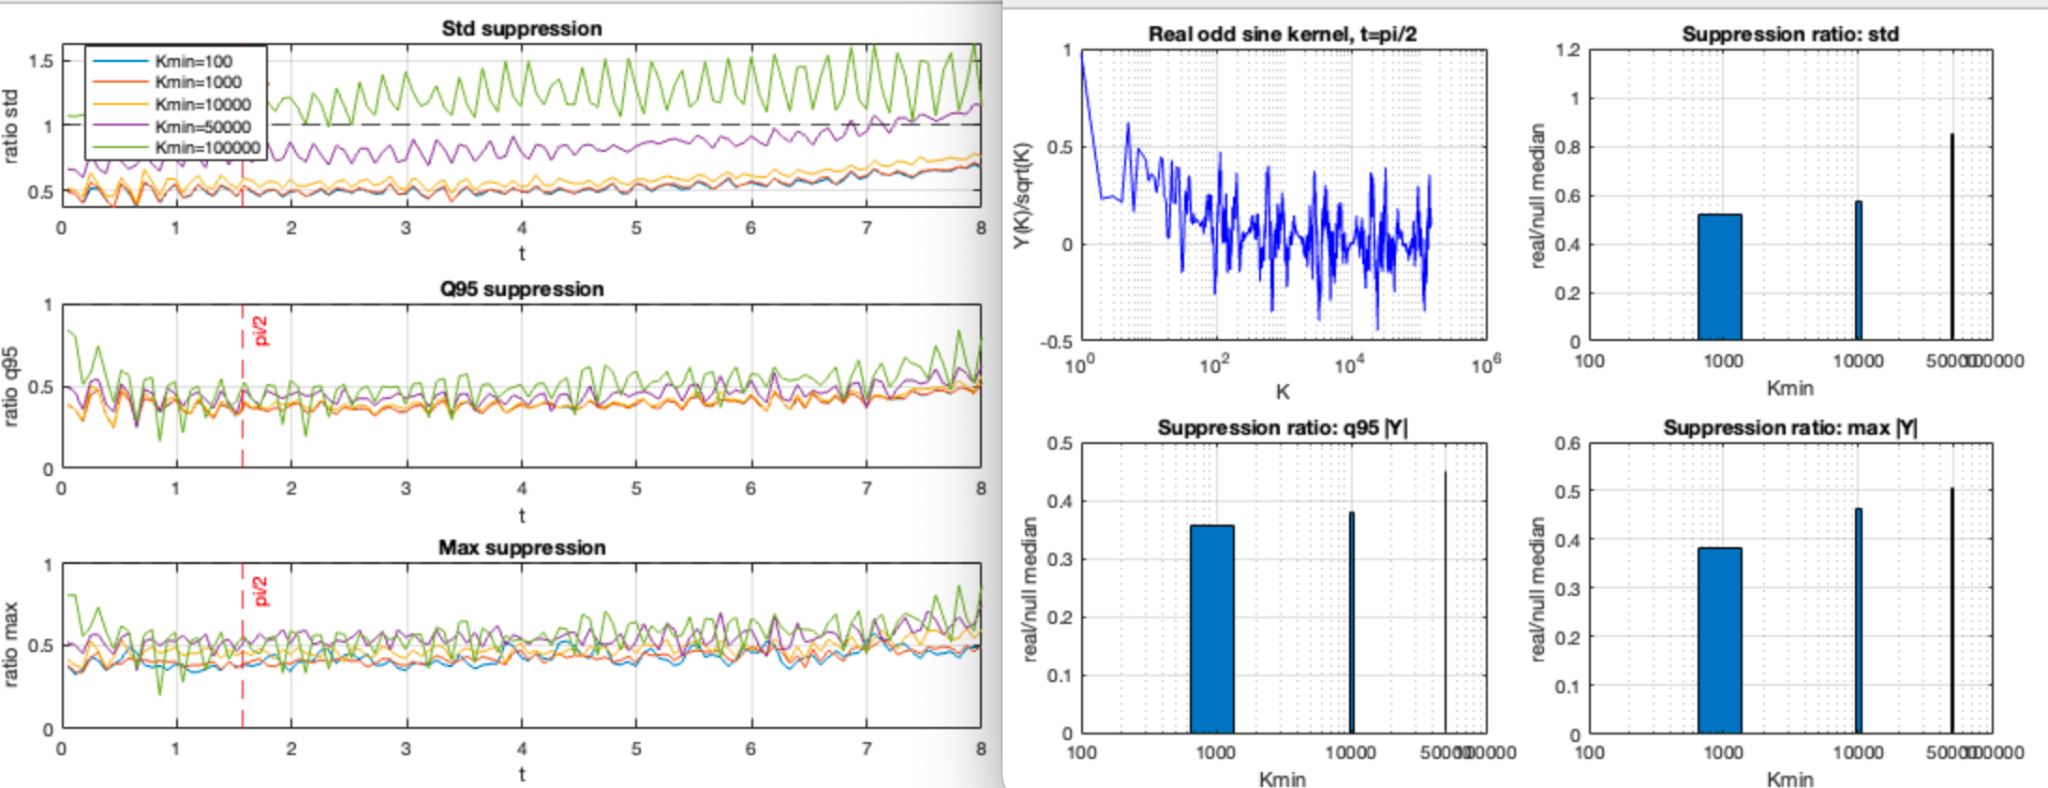
\includegraphics[width=\textwidth]{odd_sine_suppression.png}
\caption{Odd sine suppression experiment for $c=\pi/2$.  Left: sweep in
$t$ for tail statistics.  Right: one representative normalized path and
tail suppression ratios.}
\label{fig:odd_sine_suppression}
\end{figure}

The displayed frequency was chosen before the extended sweep and has no
special numerical status.  The sweep is used to motivate the analytic
study of $D_t(s)$ for general nonzero $t$.



\section{Classical statistics and variance normalization}
\label{sec:classical_statistics}

The sign-permutation experiment in Section \ref{sec:numerical_evidence}
compares the real Moebius signs with random signs preserving the
squarefree mask.  A separate test is needed to check whether the effect is
only caused by the marginal distribution of the deterministic weight
\begin{equation}
f_t(k)=\sin\bigl(t\log(c p_k)\bigr).
\label{eq:classical_ft_definition}
\end{equation}
The useful comparison is between the unweighted average of $f_t$, the
squarefree-restricted average of $\mu(k)^2f_t(k)$, and the signed average
of $\mu(k)f_t(k)$.

\begin{definition}[Variance-normalized kernel statistic]
\label{def:classical_kernel_statistics}
For $1\le k\le K$, define
\begin{equation}
Y_t(K)=\sum_{j\le K}\mu(j)f_t(j),
\label{eq:classical_YtK}
\end{equation}
\begin{equation}
V_t(K)=\sum_{j\le K}\mu(j)^2 f_t(j)^2,
\label{eq:classical_VtK}
\end{equation}
and
\begin{equation}
Z_t(K)=\frac{Y_t(K)}{\sqrt{V_t(K)}}.
\label{eq:classical_ZtK}
\end{equation}
The statistic $Z_t(K)$ measures the signed sum against the quadratic
scale generated by its own weight.
\end{definition}

The computation was extended to primes
\begin{equation}
p_k\le 2.5\cdot 10^8,
\qquad
K=13,679,318.
\label{eq:extended_statistics_K}
\end{equation}
The corresponding Moebius counts were
\begin{equation}
\#\{\mu=-1\}=4,158,169,
\quad
\#\{\mu=0\}=5,363,273,
\quad
\#\{\mu=1\}=4,157,876.
\label{eq:extended_statistics_mobius_counts}
\end{equation}
One non-optimized frequency was retained as an arbitrary reference
cross-section of the two-parameter data.  It was not selected because of
an extremal statistic; the extended sweep shows stronger low-escape
frequencies elsewhere.

\begin{experiment}[Extended classical statistics]
\label{exp:extended_classical_statistics}
At the representative frequency, the extended computation gives
\begin{align}
\frac1K\sum_{k\le K}f_t(k)&=-0.50352,
&
\frac1K\sum_{k\le K}\mu(k)^2f_t(k)&=-0.30610,
\label{eq:extended_means_unsigned}\end{align}
while the signed average is
\begin{equation}
\frac1K\sum_{k\le K}\mu(k)f_t(k)=1.3289\cdot 10^{-5}.
\label{eq:extended_mean_signed}
\end{equation}
The second moment and endpoint normalization are
\begin{equation}
\frac1K\sum_{k\le K}\mu(k)^2f_t(k)^2=0.33571,
\qquad
\sqrt{V_t(K)}=2143,
\label{eq:extended_second_moment}
\end{equation}
and
\begin{equation}
Y_t(K)=181.79,
\qquad
\frac{Y_t(K)}{\sqrt K}=0.049151,
\qquad
Z_t(K)=0.08483.
\label{eq:extended_endpoint_values}
\end{equation}
\end{experiment}

The first two averages in \eqref{eq:extended_means_unsigned} are not
small.  Thus the weight is not being centered by itself, nor by the
squarefree mask.  The signed average in \eqref{eq:extended_mean_signed}
is small only after multiplication by the Moebius signs.  This is the
basic statistic excluding the trivial explanation by marginal
equidistribution of $f_t(k)$.

\begin{experiment}[Extended tail compression]
\label{exp:extended_tail_compression}
For the same representative frequency, the tail quantiles remain stable
when the initial segment is removed.  The columns $q95_{\sqrt K}$ and
$\max_{\sqrt K}$ refer to $|Y_t(K)|/\sqrt K$ on $K\ge K_{\min}$, while
$q95_Z$ and $\max_Z$ refer to $|Z_t(K)|$ on the same tail.
\begin{table}[htbp]
\centering
\begin{tabular}{rcccc}
\hline
$K_{\min}$ & $q95_{\sqrt K}$ & $\max_{\sqrt K}$ & $q95_Z$ & $\max_Z$ \\
\hline
$100$    & $0.26111$ & $0.47049$ & $0.47445$ & $0.83065$ \\
$1000$   & $0.26111$ & $0.44661$ & $0.47443$ & $0.78534$ \\
$10000$  & $0.26112$ & $0.44661$ & $0.47445$ & $0.78534$ \\
$100000$ & $0.26114$ & $0.42119$ & $0.47437$ & $0.73218$ \\
\hline
\end{tabular}
\caption{Extended tail statistics for the odd log-prime kernel after square-root and variance normalization.}
\label{tab:extended_tail_variance_statistics}
\end{table}
\end{experiment}

The quantile statistics in Table \ref{tab:extended_tail_variance_statistics}
are essentially unchanged from $K_{\min}=100$ to $K_{\min}=100000$.
This shows that the compression is not an artifact of the first few terms.
The maximum is larger and more sensitive, as expected for an extremal
statistic, but it also decreases after removing the initial segment.



\begin{proposition}[Numerical interpretation of the extended variance test]
\label{prop:extended_variance_interpretation}
In the extended computation, the odd log-prime kernel is not suppressed
merely because $f_t(k)$ has a small marginal mean or variance.  The
suppression persists after normalization by $V_t(K)$ in
\eqref{eq:classical_VtK}, and it remains stable under tail truncation.
\end{proposition}

\begin{proof}
This is a numerical proposition based on Experiments
\ref{exp:extended_classical_statistics} and
\ref{exp:extended_tail_compression}.  The marginal averages in
\eqref{eq:extended_means_unsigned} are not close to zero, whereas the
signed average \eqref{eq:extended_mean_signed} is much smaller.  The
endpoint value in \eqref{eq:extended_endpoint_values} gives
$Z_t(K)=0.08483$, and the tail values in Table
\ref{tab:extended_tail_variance_statistics} give
$q95_Z\simeq0.474$ across the displayed truncations.  Hence the smallness
survives the intrinsic variance normalization and is not explained by the
weight alone.
\end{proof}

\begin{figure}[htbp]
\centering
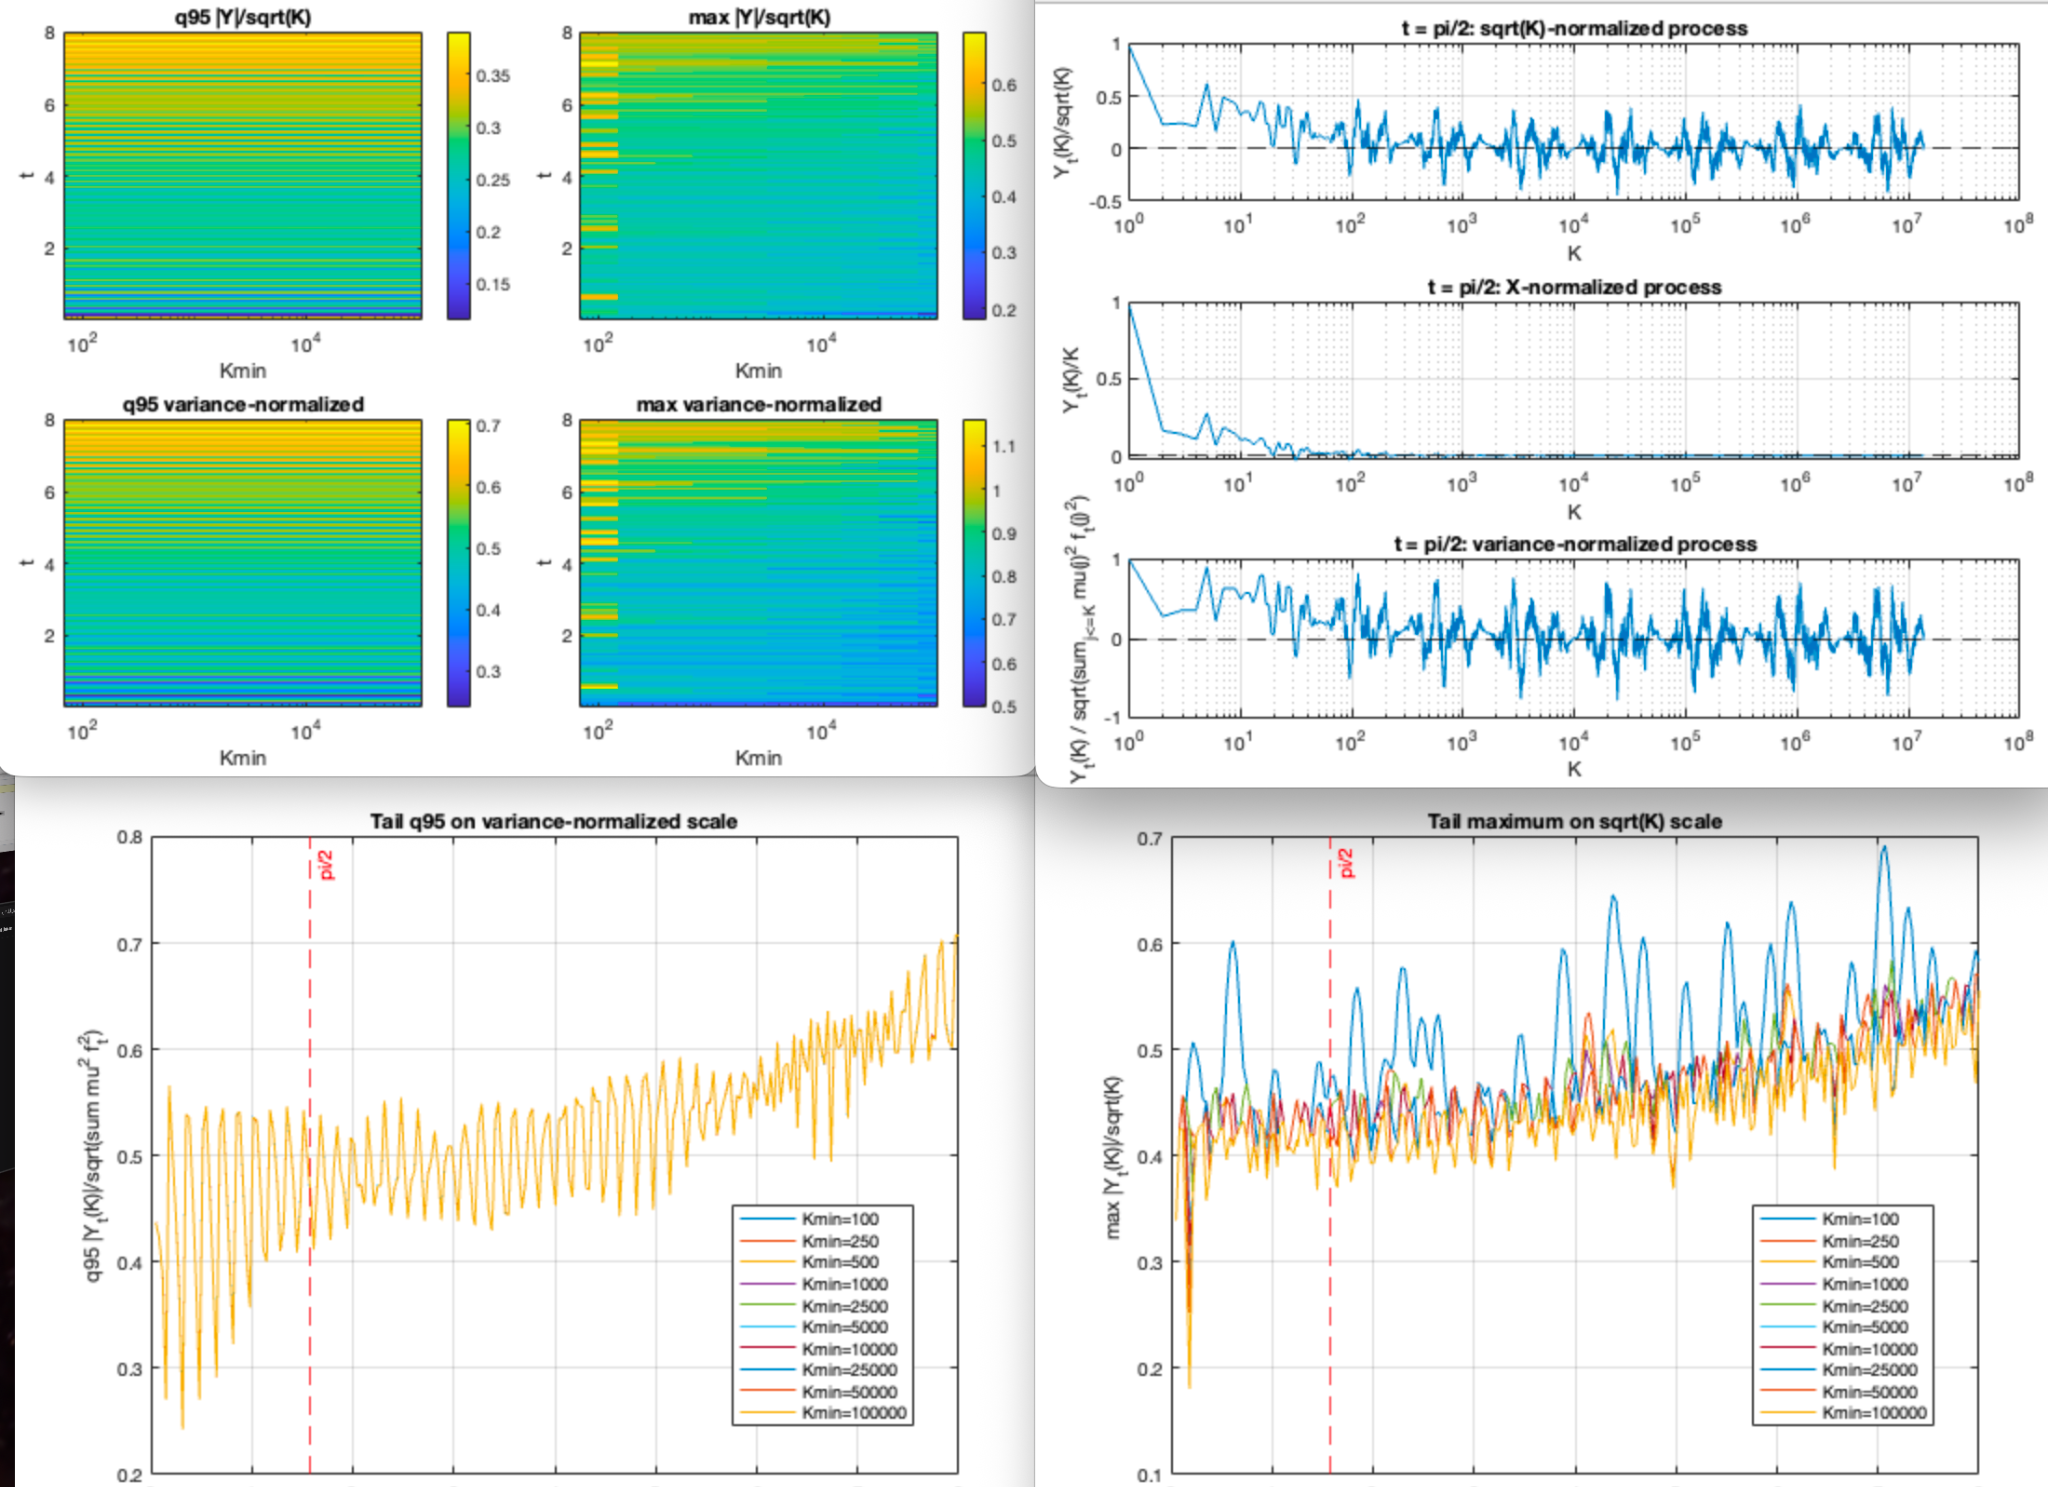
\includegraphics[width=\textwidth]{extended_statistics_dashboard.png}
\caption{Extended classical statistics for the odd log-prime Moebius
kernel up to $p_k\le 2.5\cdot10^8$.  The dashboard shows heatmaps for
tail quantiles and maxima, together with one representative normalized
path.  The variance-normalized quantiles remain compressed under tail
truncation.}
\label{fig:extended_statistics_dashboard}
\end{figure}


\begin{experiment}[Random-sign trajectory envelopes]
\label{exp:random_sign_trajectory_envelopes}
The previous statistics compress each frequency to a small number of tail
functionals.  To test whether the effect is visible at the level of the
whole path, three frequencies were then compared with random-sign walks on
the same squarefree support.  The null paths were
\begin{equation}
Y^{(r)}_t(K)=\sum_{j\le K}\varepsilon^{(r)}_j\mu(j)^2
\sin\bigl(t\log(c p_j)\bigr),
\label{eq:random_sign_null_paths}
\end{equation}
where the signs $\varepsilon^{(r)}_j\in\{-1,1\}$ are independent on the
squarefree support.  The experiment used $200$ null paths and $2231$
logarithmically spaced sample points up to $K=13,679,318$.

The extended sweep ranks $t=3.0437$, $t=0.48243$, and $t=7.8337$ among
the strongest low-escape frequencies in the tested range.  Detailed
trajectory plots were generated for $t=3.0437$, $t=0.48243$, and one
arbitrary non-optimized reference frequency.  Table
\ref{tab:trajectory_null_summary} reports the endpoint statistic and the
comparison with the null envelopes for the plotted paths.  The
columns $q95_Z$ and $\max_Z$ are computed on the tail $K\ge 10^5$; the
null columns give the median of the same statistic over the null paths.
The quantity $p_{\le}$ is the fraction of null realizations with statistic
less than or equal to the real statistic.

\begin{table}[htbp]
\centering
\small
\begin{tabular}{ccccccc}
\hline
$t$ & $Z_t(K)$ & below null median & real $q95_Z$ & null median $q95_Z$ & real $\max_Z$ & null median $\max_Z$ \\
\hline
$3.0437$ & $-0.001415$ & $0.991484$ & $0.43850$ & $1.5953$ & $0.78673$ & $1.9732$ \\
$0.48243$ & $0.004730$ & $0.981623$ & $0.27038$ & $1.5965$ & $0.71139$ & $1.9996$ \\
$1.5708$ (arb.) & $0.084830$ & $0.994621$ & $0.47437$ & $1.5919$ & $0.73218$ & $2.0142$ \\
\hline
\end{tabular}
\caption{Trajectory-level comparison with random-sign null paths on the same squarefree support.  In all three displayed cases, $p_{\le}=0$ for both $q95_Z$ and $\max_Z$ at $K_{\min}=10^5$ among the $200$ null realizations.}
\label{tab:trajectory_null_summary}
\end{table}
\end{experiment}

The table shows that the real paths are not merely ending close to zero.
They remain below the median absolute null envelope on more than $98\%$ of
the sampled points, and the tail $q95_Z$ and $\max_Z$ statistics are below
every sampled null realization at $K_{\min}=10^5$ for the three displayed
frequencies.  Thus the effect is trajectory-level compression relative to
the natural random-sign model, not just endpoint cancellation.

The extended sweep also provides a direct variance-scale summary for the
three selected low-escape frequencies.  Table~\ref{tab:selected_three_t_summary}
uses $K=13,679,318$ and reports the endpoint value in intrinsic standard
deviation units, together with tail statistics at $K_{\min}=10^5$.  For
$t=3.0437$ and $t=0.48243$, the random-sign trajectory test also gives the
median null value of the same $q95_Z$ statistic.  The value $t=7.8337$ is the
third selected low-escape frequency from the sweep; it was not included in
the trajectory-envelope plots, so only its sweep-level variance statistics
are reported.

\begin{table}[htbp]
\centering
\small
\begin{tabular}{cccccc}
\hline
$t$ & $|Z_t(K)|$ & $q95_Z$ & $\max_Z$ & null median $q95_Z$ & $q95_Z$/null median \\
\hline
$3.0437$ & $0.001415$ & $0.43850$ & $0.78673$ & $1.5953$ & $0.275$ \\
$0.48243$ & $0.004730$ & $0.27038$ & $0.71139$ & $1.5965$ & $0.169$ \\
$7.8337$ & $0.002147$ & $0.70299$ & $0.91811$ & --- & --- \\
\hline
\end{tabular}
\caption{Variance-scale cancellation for the three selected low-escape
frequencies from the extended sweep.  The endpoint statistic $|Z_t(K)|$
measures the final cancellation in units of the internal standard deviation.
The tail statistics are computed on $K\ge 10^5$.}
\label{tab:selected_three_t_summary}
\end{table}


\begin{figure}[htbp]
\centering
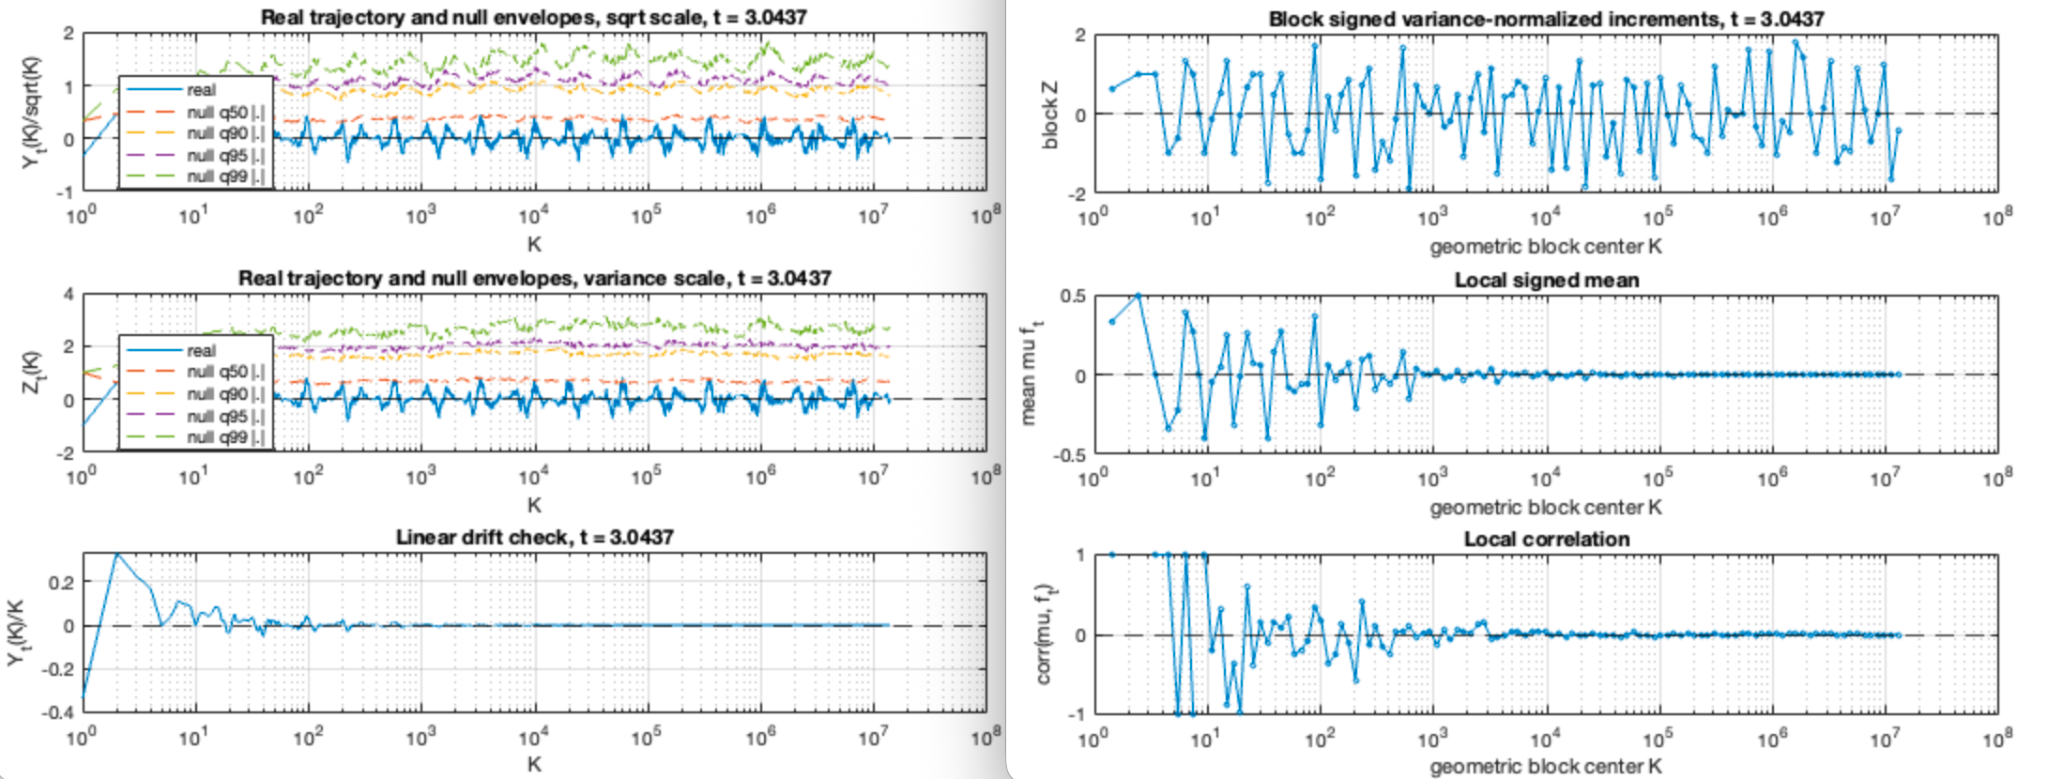
\includegraphics[width=\textwidth]{trajectory_null_t_3p0437.png}
\caption{Trajectory and local block diagnostics for the low-escape
frequency $t=3.0437$.  Left: real path compared with random-sign absolute
null envelopes on the $\sqrt K$ scale and on the intrinsic variance scale.
Right: logarithmic block diagnostics.  The path remains below the typical
null envelopes even though the signed block increments fluctuate on a
normal local scale.}
\label{fig:trajectory_null_t_3p0437}
\end{figure}

\begin{figure}[htbp]
\centering
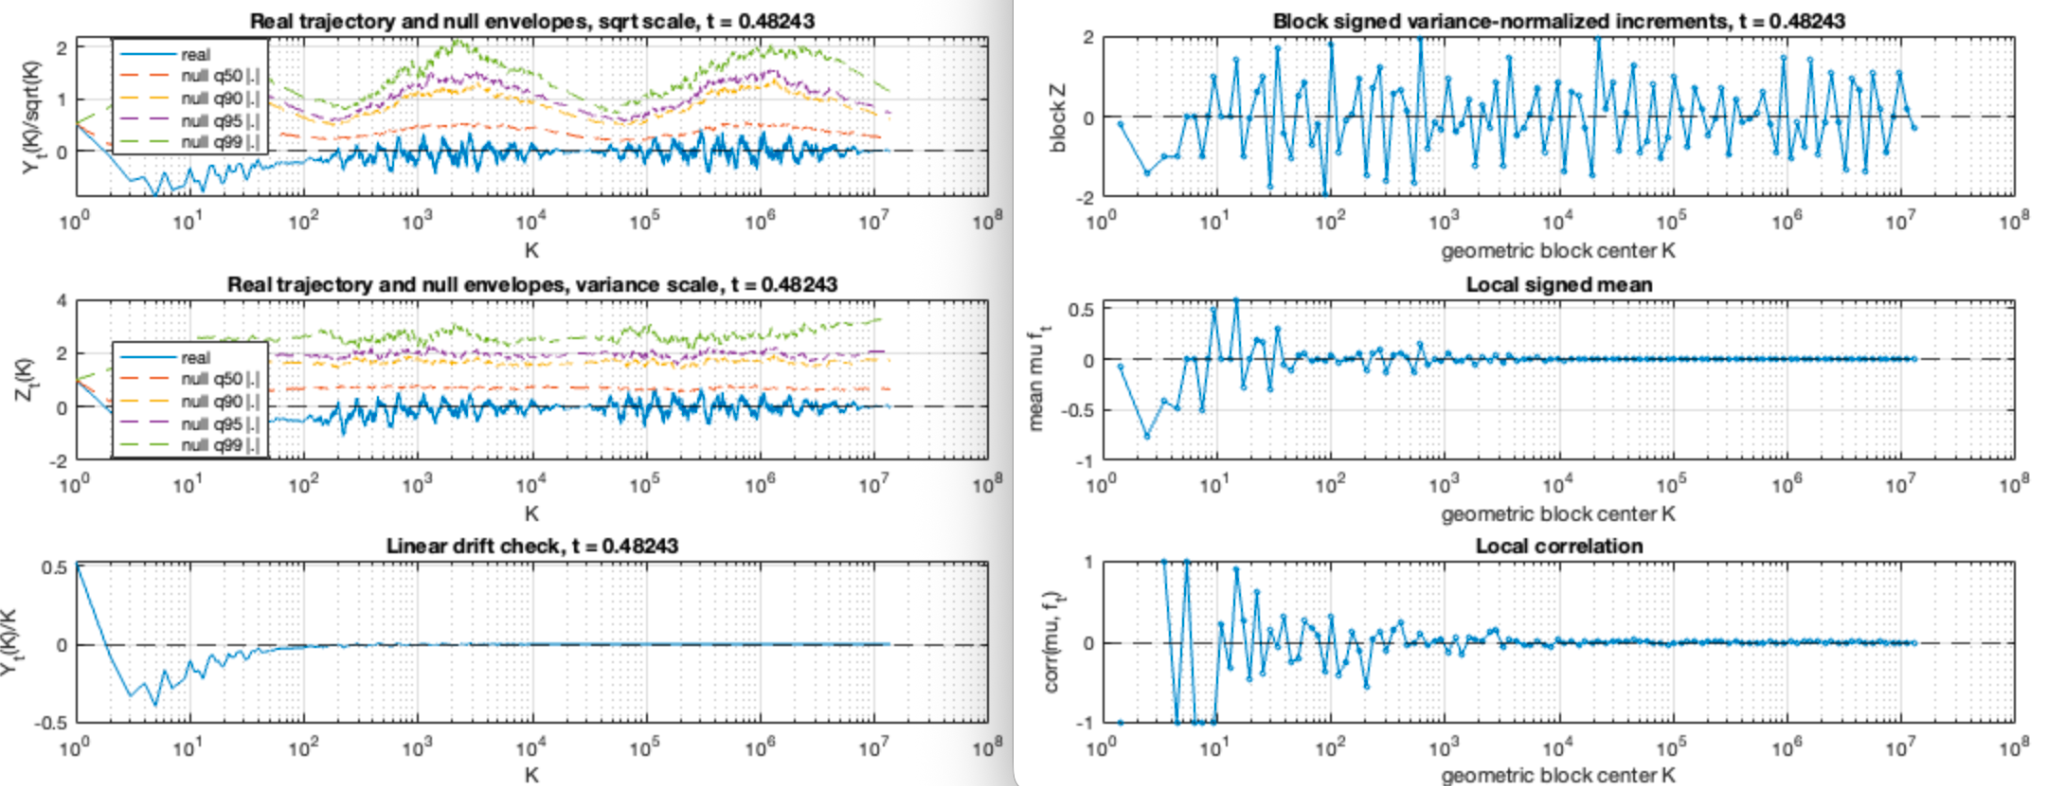
\includegraphics[width=\textwidth]{trajectory_null_t_0p48243.png}
\caption{Trajectory and local block diagnostics for the low-escape
frequency $t=0.48243$.  The real trajectory is again compressed relative
to random-sign walks with the same support and deterministic weight.  The
linear drift diagnostic tends rapidly to zero.}
\label{fig:trajectory_null_t_0p48243}
\end{figure}

\begin{figure}[htbp]
\centering
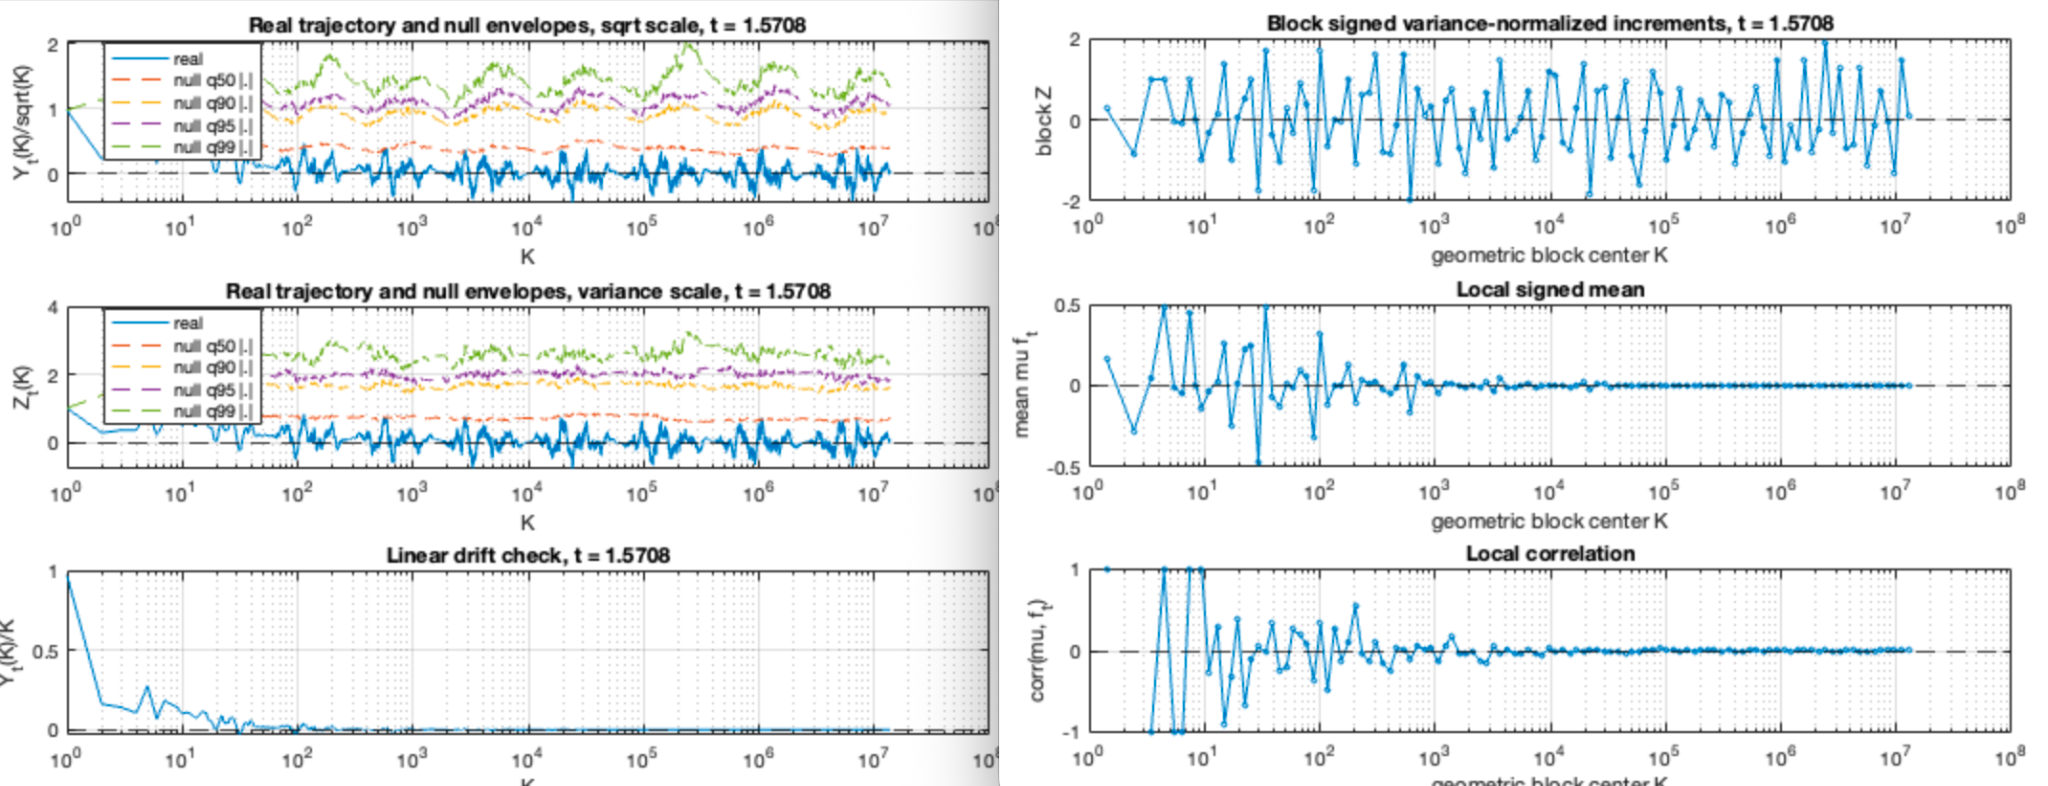
\includegraphics[width=\textwidth]{trajectory_null_t_reference.png}
\caption{Trajectory and local block diagnostics for the non-optimized
arbitrary reference frequency $t=1.5708$.  Its role is only to show that
the compression is not confined to frequencies selected by an extremal
sweep.}
\label{fig:trajectory_null_t_reference}
\end{figure}

\begin{proposition}[Numerical interpretation of the trajectory null test]
\label{prop:trajectory_null_interpretation}
In the extended computation, the low-escape behavior is visible as a
compressed trajectory relative to random signs on the same squarefree
support.  It is not only an endpoint cancellation and not a consequence of
uniformly small local blocks.
\end{proposition}

\begin{proof}
The endpoint values alone would not distinguish a persistent low-escape
path from a late accidental crossing.  Experiment
\ref{exp:random_sign_trajectory_envelopes} compares the whole sampled path
with the envelopes generated by \eqref{eq:random_sign_null_paths}.  For
$t=3.0437$, $0.48243$, and the arbitrary reference frequency, the real
path is below the null median on respectively $0.991484$, $0.981623$, and
$0.994621$ of the sample grid.  At $K_{\min}=10^5$, both the tail quantile
$q95_Z$ and the tail maximum $\max_Z$ have $p_{\le}=0$ among $200$ null
realizations for all three displayed frequencies.  Hence the compression is
seen throughout the path and in the tail functionals, not only at the final
point.  The block plots in Figures \ref{fig:trajectory_null_t_3p0437}--
\ref{fig:trajectory_null_t_reference} show signed block increments of order
one; therefore the observed effect should be interpreted as unusually small
long-range escape of ordinary local fluctuations, rather than as uniform
local annihilation block by block.
\end{proof}

The statistical conclusion is that the observed smallness is a property of
the signed product
\begin{equation}
\mu(k)\sin\bigl(t\log(c p_k)\bigr),
\label{eq:signed_product_conclusion}
\end{equation}
not of the deterministic factor alone.  The trajectory-level null test
strengthens this conclusion: the real Moebius signs produce paths with
substantially less escape than random signs on the same squarefree support.
This supports the use of the Dirichlet series $D_t(s)$ in
\eqref{eq:Dt_definition} as the analytic object attached to the kernel.

\section{Conclusion}
\label{sec:conclusion}

The main purpose of this work has been to exhibit finite-range cancellation
for the odd log-prime kernel
\begin{equation}
Y_t(X)=\sum_{k\le X}\mu(k)\sin(t\log(c p_k))
\label{eq:conclusion_kernel}
\end{equation}
and to isolate the analytic conditions under which this cancellation would
extend to an asymptotic regime.  The kernel leads to the Dirichlet series
\begin{equation}
D_t(s)=\sum_{k\ge1}\frac{\mu(k)\sin(t\log(c p_k))}{k^s}.
\label{eq:conclusion_Dt}
\end{equation}
A square-root scale estimate for \eqref{eq:conclusion_kernel} implies, by
Abelian continuation, holomorphy of \eqref{eq:conclusion_Dt} beyond the
critical boundary.

The local singularity transfer carried out in Section~\ref{sec:singularity_transfer}
shows how the exact prime-index factor $p_k^{\pm it}$ inherits the leading
singular branches of the shifted reciprocal zeta factors.  For a simple
zero $\rho$ of $\zeta$, the inherited branches occur at
\begin{equation}
s=\rho+it
\label{eq:conclusion_plus_branch_location}
\end{equation}
and
\begin{equation}
s=\rho-it,
\label{eq:conclusion_minus_branch_location}
\end{equation}
with leading coefficients
\begin{equation}
\frac{c^{it}\Gamma(1+it)}{2i\,\zeta'(\rho)}
\label{eq:conclusion_plus_branch_coefficient}
\end{equation}
and
\begin{equation}
-\frac{c^{-it}\Gamma(1-it)}{2i\,\zeta'(\rho)}.
\label{eq:conclusion_minus_branch_coefficient}
\end{equation}
The explicit Cipolla corrections to $p_k$ have lower local singular order.
The strong fractional transfer hypothesis isolates the remaining analytic
requirement: the exact logarithmic remainder of the prime-index symbol must
also be locally lower order and must not reconstruct the leading branch.

The numerical experiments for fixed $c$ give a finite-range test of this
mechanism.  In the extended sweep through the first $225$ evaluated
frequencies, the selected low-escape values are
\begin{equation}
t=3.0437,
\qquad
 t=0.48243,
\qquad
 t=7.8337.
\label{eq:conclusion_selected_frequencies}
\end{equation}
At $p_k\le 2.5\cdot10^8$, the corresponding endpoint cancellation on the
intrinsic variance scale is
\begin{equation}
|Z_t(K)|=0.001415,
\qquad
|Z_t(K)|=0.004730,
\qquad
|Z_t(K)|=0.002147,
\label{eq:conclusion_selected_Z_values}
\end{equation}
respectively.  The detailed random-sign trajectory tests for the first two
selected frequencies show that the real paths remain compressed relative to
null walks on the same squarefree support and with the same deterministic
weight.  The effect is therefore not only endpoint cancellation and is not
explained by the marginal distribution of the phase weight alone.

The strong fractional transfer hypothesis that emerges from this analysis
does not follow, at least trivially, from the Riemann Hypothesis.  RH imposes
global restrictions on the location of zeros, but it does not by itself
guarantee the local analytic stability, symbolic logarithmic transfer, or
microlocal non-cancellation required by the mechanism above.  Consequently,
even if RH is true, the analytic condition identified here retains separate
content.

Under the strong transfer hypothesis and a square-root bound for
$Y_t(X)$, Theorem~\ref{thm:conditional_link_RH} forces every simple
nontrivial zero of $\zeta(s)$ onto the critical line.  Thus the paper reduces
the conditional route to two explicit requirements: local symbolic transfer
for the exact prime-index logarithmic factor, and square-root cancellation
for the odd log-prime kernel.

\begin{thebibliography}{99}


\bibitem{Cipolla1902}
M. Cipolla,
\emph{La determinazione assintotica dell' nimo numero primo},
Napoli Rendiconti \textbf{8} (1902), 132--166.

\bibitem{AriasToulisse2013}
J. Arias de Reyna and J. Toulisse,
\emph{The $n$-th prime asymptotically},
Journal de Th\'eorie des Nombres de Bordeaux \textbf{25} (2013), no. 3,
521--555.
doi:10.5802/jtnb.847.

\bibitem{Davenport2000}
H. Davenport,
\emph{Multiplicative Number Theory},
3rd ed., revised by H. L. Montgomery,
Graduate Texts in Mathematics, vol. 74, Springer, 2000.
doi:10.1007/978-1-4757-5927-3.

\bibitem{Edwards2001}
H. M. Edwards,
\emph{Riemann's Zeta Function},
Dover Publications, Mineola, NY, 2001.
ISBN: 978-0486417400.

\bibitem{IwaniecKowalski2004}
H. Iwaniec and E. Kowalski,
\emph{Analytic Number Theory},
American Mathematical Society Colloquium Publications, vol. 53,
American Mathematical Society, Providence, RI, 2004.
doi:10.1090/coll/053.

\bibitem{MontgomeryVaughan2007}
H. L. Montgomery and R. C. Vaughan,
\emph{Multiplicative Number Theory I: Classical Theory},
Cambridge Studies in Advanced Mathematics, vol. 97,
Cambridge University Press, 2007.
doi:10.1017/CBO9780511618314.

\bibitem{OdlyzkoTeRiele1985}
A. M. Odlyzko and H. J. J. te Riele,
\emph{Disproof of the Mertens conjecture},
Journal f\"ur die reine und angewandte Mathematik \textbf{1985} (1985),
no. 357, 138--160.
doi:10.1515/crll.1985.357.138.

\bibitem{RosserSchoenfeld1962}
J. B. Rosser and L. Schoenfeld,
\emph{Approximate formulas for some functions of prime numbers},
Illinois Journal of Mathematics \textbf{6} (1962), no. 1, 64--94.
doi:10.1215/ijm/1255631807.

\bibitem{Titchmarsh1986}
E. C. Titchmarsh,
\emph{The Theory of the Riemann Zeta-Function},
2nd ed., revised by D. R. Heath-Brown,
Oxford University Press, 1986.
ISBN: 978-0198533696.

\end{thebibliography}

\end{document}
